\chapter{المخططات التنظيمية والسلف المشترك}\label{ch:g10:common-ancestry}

مُدَّ ذراعك وعُدّ: عظم واحد من الكتف إلى المرفق، وعظمان من المرفق إلى
الرسغ، وحفنة من العظام الصغيرة في الرسغ، وخمس أصابع. ثم انظر إلى هيكل
جناح خفاش، وزعنفة حوت، وطرف حصان الأمامي، وذراع ضفدع: العظم الواحد
نفسه، والعظمان، والحفنة، والأصابع، ممدودة أو ملتحمة أو مقصّرة لكنها لم
يعد ترتيبها قط. وما كان أحد يصمم جناحًا من جديد ليبدأ من ذراع. فالشبه
علامة على شيء موروث، وهذا الفصل عن قراءة تلك العلامات --- في الهياكل،
وفي الأجنة، وفي الجزيئات --- لإعادة بناء قرابة الكائنات الحية.

\section{المخطط التنظيمي للفقاريات}

\begin{definition}[المخطط التنظيمي]\label{def:g10:common-ancestry:bodyplan}
\emph{المخطط التنظيمي}\index{مخطط تنظيمي} لمجموعة من الكائنات هو
الترتيب المشترك لأجزائها: محاور التناظر والمواضع النسبية للأعضاء
الرئيسية، بصرف النظر عن الحجم والشكل ونمط العيش. و\emph{الفقاريات}
\index{فقاري} --- أسماك وبرمائيات وزواحف وطيور وثدييات --- تتقاسم
مخططًا واحدًا: جسم متناظر حول مستوٍ شاقولي، له طرف أمامي يحمل الرأس
وطرف خلفي؛ وهيكل داخلي محوره عمود من الفقرات يحمي حبلًا عصبيًا ظهريًا؛
وأنبوب هضمي يمتد بطنيًا، والفم في المقدمة، والقلب تحته.
\end{definition}

\begin{omfigure}
\begin{tikzpicture}[font=\small, >=Stealth]
  % generic vertebrate side view
  \draw[thick, fill=omDef!6, rounded corners=14pt] (0,0) rectangle (9,3.2);
  \draw[thick, omThm] (0.6,2.5) -- (8.6,2.5);                      % nerve cord
  \foreach \x in {1.2,1.8,...,8.4} \draw[thick] (\x,2.15) -- (\x,2.35); % vertebrae
  \draw[thick] (1.0,2.25) -- (8.6,2.25);
  \draw[thick, omProp, fill=omProp!20] (0.5,1.4) .. controls (2,0.7) and (6,0.7) .. (8.6,1.2)
    .. controls (6,1.5) and (2,1.9) .. (0.5,1.4);                      % gut
  \draw[thick, omThm, fill=omThm!30] (2.3,0.75) circle (0.32);         % heart
  \node[anchor=west] at (9.4,2.5) {الحبل العصبي (ظهري)};
  \draw[->] (9.35,2.5) -- (8.65,2.5);
  \node[anchor=west] at (9.4,2.0) {العمود الفقري};
  \draw[->] (9.35,2.0) -- (8.6,2.22);
  \node[anchor=west] at (9.4,1.2) {الأنبوب الهضمي (بطني)};
  \draw[->] (9.35,1.2) -- (8.65,1.2);
  \node[anchor=north] at (2.3,-0.1) {القلب، تحت الأنبوب};
  \draw[->] (2.3,-0.05) -- (2.3,0.4);
  \node[anchor=east] at (-0.1,1.4) {الفم};
  \draw[->] (-0.05,1.4) -- (0.45,1.4);
  \node[anchor=south, font=\small\itshape] at (4.5,3.3) {الجهة الظهرية};
  \node[anchor=north, font=\small\itshape] at (6.5,-0.05) {الجهة البطنية};
  \draw[<->, gray] (0,3.7) -- (9,3.7) node[midway, above, font=\scriptsize] {محور الأمام والخلف};
\end{tikzpicture}

{\small \omterm{def:g10:common-ancestry:bodyplan}{المخطط التنظيمي} للفقاريات، من الجانب. أيًّا كان \omterm{def:g10:biodiversity-scales:species}{النوع}، يمتد
الحبل العصبي على طول الظهر فوق العمود الفقري، ويمتد الأنبوب الهضمي على
طول البطن، ويقع القلب تحته قرب المقدمة. أما الحشرات وديدان الأرض
فحبلها العصبي في الجهة البطنية: وذلك مخطط آخر.}
\end{omfigure}

\begin{example}[المخطط نفسه، حيوانات مختلفة]\label{ex:g10:common-ancestry:sameplan}
تشريح سلمون مرقط وضفدع وسحلية وحمامة وفأر جنبًا إلى جنب يبين المخطط في
كل حالة: النخاع الشوكي في الظهر تحميه الفقرات؛ والمعي تحته وإلى جانب
المعدة كبد؛ والقلب في المقدمة تحت المعي؛ وأطراف مزدوجة (أو زعانف) تصل
بأحزمة من العظم. أما الفروق --- غلاصم أو رئات، وزعانف أو أرجل، وحراشف
أو ريش أو فرو --- فكلها صور مبنية على الترتيب نفسه.
\end{example}

\section{الأعضاء المتماثلة}

\begin{definition}[التماثل]\label{def:g10:common-ancestry:homology}
عضوان في نوعين \emph{متماثلان}\index{تماثل} إذا كانت لهما البنية نفسها
والموضع نفسه في \omterm{def:g10:common-ancestry:bodyplan}{المخطط التنظيمي} --- أي مبنيان من الأجزاء نفسها في
العلاقات نفسها --- أيًّا كانت وظيفتهما الحالية. والأطراف الأمامية
لرباعيات الأطراف هي المثال المعياري: عظم واحد (العضد)، وعظمان (الكعبرة
والزند)، وحفنة من عظام الرسغ، ثم الأصابع. أما الأعضاء التي تؤدي
الوظيفة نفسها ببنية مختلفة --- كجناح الطائر وجناح الذبابة --- فليست
إلا \emph{متشابهة}، ولا تقول شيئًا عن القرابة.
\end{definition}

\begin{omfigure}
\begin{tikzpicture}[font=\small, line cap=round]
  % three stylised forelimbs: humerus (red), radius+ulna (blue), carpals (gray), digits (green)
  \tikzset{hum/.style={line width=6pt, omThm!70},
           ru/.style={line width=4pt, omDef!70},
           carp/.style={fill=gray!50, draw=gray!70},
           dig/.style={line width=3pt, omMeth!80}}
  % human arm
  \begin{scope}
    \draw[hum] (0,3.2) -- (0.2,1.9);
    \draw[ru] (0.1,1.85) -- (0.3,0.9); \draw[ru] (0.35,1.85) -- (0.5,0.9);
    \fill[carp] (0.15,0.7) rectangle (0.65,0.85);
    \foreach \dx in {-0.3,-0.12,0.05,0.22,0.4} \draw[dig] (0.4,0.7) -- ({0.4+\dx},-0.1);
    \node[anchor=north] at (0.4,-1.4) {ذراع إنسان};
  \end{scope}
  % bat wing
  \begin{scope}[xshift=3.6cm]
    \draw[hum] (0,3.2) -- (0.4,2.3);
    \draw[ru] (0.4,2.3) -- (1.0,1.3);
    \fill[carp] (0.95,1.2) rectangle (1.25,1.35);
    \draw[dig] (1.1,1.2) -- (0.8,0.9);
    \foreach \a in {-0.6,-0.3,0.1,0.5} \draw[dig] (1.1,1.2) -- ({1.1+2.2*cos(-60+40*\a)},{1.2+2.2*sin(-60+40*\a)});
    \node[anchor=north] at (1.2,-1.4) {جناح خفاش};
  \end{scope}
  % whale flipper
  \begin{scope}[xshift=8.0cm]
    \draw[hum] (0,3.2) -- (0.1,2.5);
    \draw[ru] (0.0,2.45) -- (0.05,1.9); \draw[ru] (0.3,2.45) -- (0.35,1.9);
    \fill[carp] (-0.05,1.6) rectangle (0.5,1.85);
    \foreach \dx in {-0.2,0.0,0.2,0.45} \draw[dig] ({0.22+0.5*\dx},1.6) -- ({0.22+\dx},0.2);
    \draw[gray!60, rounded corners=8pt] (-0.5,3.4) -- (-0.6,0.0) -- (0.9,-0.1) -- (0.9,3.4);
    \node[anchor=north] at (0.2,-1.4) {زعنفة حوت};
  \end{scope}
  % legend
  \begin{scope}[xshift=10.4cm, yshift=2.2cm]
    \draw[hum] (0,1.0) -- (0.6,1.0); \node[anchor=west] at (0.7,1.0) {العضد};
    \draw[ru] (0,0.5) -- (0.6,0.5); \node[anchor=west] at (0.7,0.5) {الكعبرة والزند};
    \fill[carp] (0.05,-0.08) rectangle (0.55,0.08); \node[anchor=west] at (0.7,0) {عظام الرسغ};
    \draw[dig] (0,-0.5) -- (0.6,-0.5); \node[anchor=west] at (0.7,-0.5) {الأصابع};
  \end{scope}
\end{tikzpicture}

{\small ثلاثة أطراف أمامية متماثلة، تخطيطيًا: العظام نفسها بالترتيب
نفسه، ممدودة جناحًا، مسطحة زعنفة. فالوظيفة تختلف؛ أما البنية والموضع
فلا.}
\end{omfigure}

\begin{omfigure}
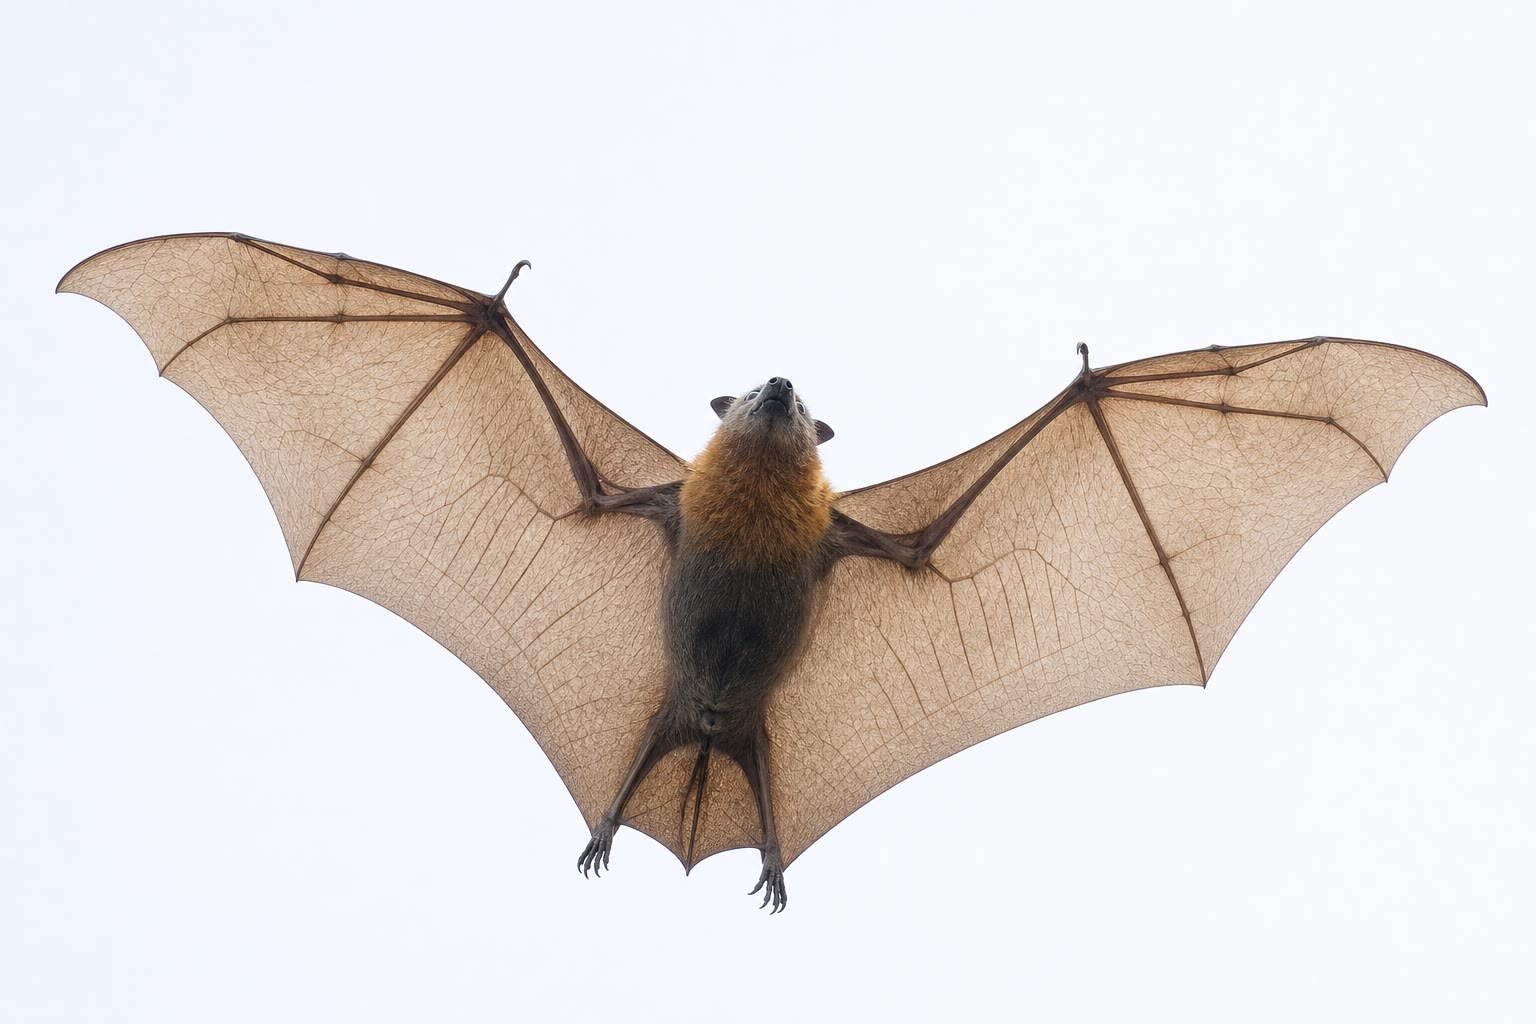
\includegraphics[width=0.6\linewidth]{images/book2/ai/g10-ancestry-bat-wing.jpg}

{\small خفاش في الطيران: غشاء الجناح مشدود على عظام أصابع استطالت
استطالة هائلة. إنها يد المخطط الثديي، وقد صارت جناحًا.}
\end{omfigure}

\begin{proposition}[التماثل يكشف القرابة]\label{prop:g10:common-ancestry:kinship}
البنى المتماثلة المشتركة موروثة من سلف مشترك كان يملكها؛ وكلما تقاسم
نوعان بنى من هذا \omterm{def:g10:biodiversity-scales:species}{النوع} أكثر، كانت قرابتهما أقرب. فطرف رباعيات الأطراف
يوجد في كل \omterm{def:g10:common-ancestry:bodyplan}{فقاري} بري لأنها جميعًا تنحدر من سلالة سلفية كانت تملكه؛
وجناح الخفاش ذراع معدلة لأن الخفافيش تنحدر من ثدييات ذوات أذرع، لا من
الطيور.
\end{proposition}
\begin{proof}[شواهد]
تتلاقى ثلاثة خطوط مستقلة. \emph{الأحافير}: فتتابع الصخور المؤرخة يحوي
صورًا بتراكيب وسيطة من الصفات --- أسماك لها زعانف تشبه الأطراف
ولها رقبة قبل 375 مليون سنة، ثم حيوانات لها أربعة أرجل ولها أذناب
تشبه أذناب الأسماك؛
ومنها أيضًا \emph{Archaeopteryx}، وعمره 150 مليون سنة، بريش وجناحين لكن أيضًا
بأسنان وأصابع مخلبية وذنب عظمي طويل. \emph{الأجنة}: فكل أجنة \omterm{def:g10:common-ancestry:bodyplan}{الفقاريات}
تمر بطور فيه جيوب غلصمية وذنب وحبل ظهري --- وهي بنى تبقى في السمكة
البالغة، وتعاد صياغتها أو تفقد عند غيرها. \emph{الجزيئات}: فكما بيّن
\cref{ch:g10:universal-dna}، تتقاسم جميعًا \omterm{def:g10:universal-dna:information}{DNA} \omterm{def:g10:universal-dna:gene}{والمورّثات} نفسها،
والفروق بين نسخ \omterm{def:g10:universal-dna:gene}{مورّثة} واحدة ترتب \omterm{def:g10:biodiversity-scales:species}{الأنواع} كما يرتبها التشريح تمامًا.
\end{proof}

\begin{omfigure}
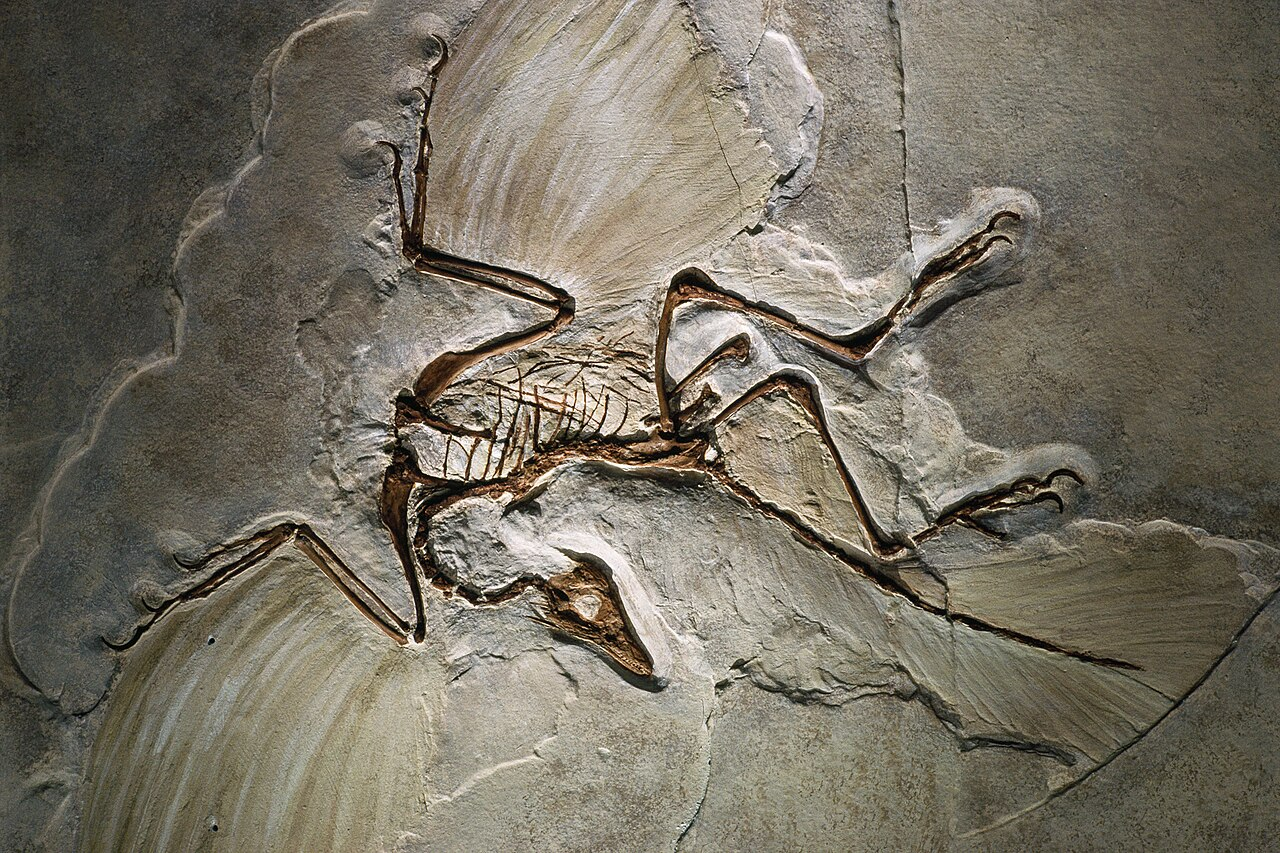
\includegraphics[width=0.5\linewidth]{images/book1/archaeopteryx.jpg}

{\small \emph{Archaeopteryx}، وعمره 150 مليون سنة: جناحان مريشان
وترقوة ملتحمة كالطائر، وأسنان وأصابع مخلبية وذنب عظمي طويل كالديناصور
الصغير. وأحفورة تجمع صفات مجموعتين هي ما يتنبأ به السلف المشترك.
تصوير جيمس ل.~آموس، CC0.}
\end{omfigure}

\section{المجموعات المتداخلة}

\begin{method}[التجميع بالصفات المشتركة]\label{met:g10:common-ancestry:grouping}
تبنى مجموعات القرابة بالصفات \emph{المشتقة} المشتركة --- أي السمات
التي ظهرت مرة واحدة في سلف وورثها كل نسله.
\begin{enumerate}
  \item اسرد \omterm{def:g10:biodiversity-scales:species}{الأنواع} ومجموعة من الصفات (عمود فقري؛ أربعة أطراف؛ بيضة
        ذات قشرة أو ما يعادلها، وهي البيضة السلوية؛ ريش؛ شعر ولبن؛ وهكذا).
  \item دوّن لكل صفة أي \omterm{def:g10:biodiversity-scales:species}{الأنواع} تملكها.
  \item الصفة التي تتقاسمها مجموعة جزئية تعرّف مجموعة: فكل \omterm{def:g10:biodiversity-scales:species}{الأنواع} ذوات
        الأطراف الأربعة هي رباعيات الأطراف؛ ومنها كل ذوات البيضة
        السلوية هي السلويات؛ ومن هذه كل ذوات الشعر هي الثدييات.
  \item ارسم المجموعات صناديق متداخلة، أو شجرة كل عقدة فيها هي السلف
        المشترك الذي ظهرت فيه الصفة. ويجب أن تحوي المجموعة \emph{كل}
        نسل ذلك السلف: و«الأسماك» أو «الزواحف» بالمعنى الدارج ليست
        مجموعات من هذا القبيل.
\end{enumerate}
\end{method}

\begin{omfigure}
\begin{tikzpicture}[font=\small]
  \node[draw, rounded corners, thick, fill=omDef!6, minimum width=12.2cm, minimum height=4.6cm] (v) at (0,0) {};
  \node[anchor=north west] at (v.north west) {\ \textbf{الفقاريات}: عمود فقري};
  \node[anchor=south west] at (v.south west) {\ سلمون مرقط};
  \node[draw, rounded corners, thick, fill=omMeth!8, minimum width=9.6cm, minimum height=3.5cm] (t) at (0.9,-0.25) {};
  \node[anchor=north west] at (t.north west) {\ \textbf{رباعيات الأطراف}: أربعة أطراف};
  \node[anchor=south west] at (t.south west) {\ ضفدع};
  \node[draw, rounded corners, thick, fill=omProp!10, minimum width=7.0cm, minimum height=2.4cm] (a) at (1.8,-0.5) {};
  \node[anchor=north west] at (a.north west) {\ \textbf{السلويات}: بيضة سلوية};
  \node[anchor=south west] at (a.south west) {\ سحلية\quad حمامة};
  \node[draw, rounded corners, thick, fill=omThm!10, minimum width=3.7cm, minimum height=1.3cm] (m) at (3.2,-0.75) {};
  \node[anchor=north west] at (m.north west) {\ \textbf{الثدييات}: شعر ولبن};
  \node[anchor=south west] at (m.south west) {\ فأر\quad إنسان};
\end{tikzpicture}

{\small مجموعات القرابة المتداخلة لخمسة فقاريات. كل صندوق تعرّفه صفة
ظهرت مرة واحدة، في السلف المشترك لكل ما بداخله. والحمامة داخل
«السلويات» مع السحلية: فالسحلية أقرب قرابة إلى الحمامة منها إلى
الضفدع.}
\end{omfigure}

\begin{example}[قراءة الصناديق]\label{ex:g10:common-ancestry:reading}
أي أقرباء الفأر أقرب إليه بين السلمون المرقط والضفدع والسحلية
والحمامة؟ أصغر صندوق يحوي الفأر ونوعًا آخر هو «السلويات»، وفيه
السحلية والحمامة: فهما على القرب نفسه، وكلاهما أقرب إلى الفأر من
الضفدع، والضفدع أقرب من السلمون. وأن تكون السحلية أقرب إلى الحمامة
منها إلى الضفدع يفاجئ معظم الناس؛ لكن البيضة ذات القشرة، وهي صفة لا
يملكها ضفدع، تحسم الأمر.
\end{example}

\section{القرابة في الجزيئات}

\begin{proposition}[القرابة الجزيئية]\label{prop:g10:common-ancestry:molecular}
لما كانت الكائنات الحية كلها تنحدر من أسلاف مشتركين، كانت \omterm{def:g10:universal-dna:gene}{المورّثة}
الموجودة في نوعين نسخة معدلة من \omterm{def:g10:universal-dna:gene}{المورّثة} السلفية، وكان عدد الفروق بين
النسختين ينمو مع الزمن المنقضي منذ افترق النوعان. فمقارنة متتالية
\omterm{def:g10:universal-dna:gene}{مورّثة} واحدة، أو \omterm{def:g10:chemistry-of-life:families}{البروتين} الذي ترمز له، عبر \omterm{def:g10:biodiversity-scales:species}{الأنواع} تقيس إذن القرابة،
والتجميعات الناتجة توافق تلك المستخرجة من التشريح.
\end{proposition}
\admitted

\begin{example}[السيتوكروم c]\label{ex:g10:common-ancestry:cytochrome}
السيتوكروم c \omterm{def:g10:chemistry-of-life:families}{بروتين} من نحو 104 حموض أمينية تستعمله كل حقيقيات \omterm{def:g10:cells-common-unit:organelle}{النواة}
في التنفس. وبمقارنته بالمتتالية البشرية، يختلف عند الشمبانزي في 0
موضع، وعند الفأر في 9، وعند الدجاجة في 13، وعند الضفدع في 18، وعند
التونة في 21، وعند الخميرة في 45. وبترتيب \omterm{def:g10:biodiversity-scales:species}{الأنواع} حسب الفروق، تقع في
صناديق الشكل السابق بالضبط: ثدييات، ثم سلويات، ثم رباعيات أطراف، ثم
فقاريات، ثم حقيقيات \omterm{def:g10:cells-common-unit:organelle}{نواة}.
\end{example}

\begin{remark}[الوحدة والقرابة]\label{rem:g10:common-ancestry:unity}
وحدة التركيب (\cref{ch:g10:chemistry-of-life})، ووحدة \omterm{def:g10:cells-common-unit:cell}{الخلية}
(\cref{ch:g10:cells-common-unit})، ووحدة الجزيء الوراثي
(\cref{ch:g10:universal-dna})، والآن وحدة المخططات التنظيمية
ومتتاليات \omterm{def:g10:universal-dna:gene}{المورّثات}: حقيقة واحدة رئيت أربع مرات: الكائنات الحية يشبه
بعضها بعضًا لأنها قريبة، وهي قريبة لأنها تنحدر من أسلاف مشتركين. وتنوع
\cref{ch:g10:biodiversity-scales} هو حصيلة ذلك الانحدار مع التعديل،
على مدى الزمن الذي يقيسه السجل الأحفوري. أما كيف تنشأ التعديلات وكيف
تنتشر فموضوع السنة الأخيرة.
\end{remark}

\section{تمارين}

\begin{exercise}[$\star$]\label{exo:g10:common-ancestry:1}
اذكر أربع سمات من \omterm{def:g10:common-ancestry:bodyplan}{المخطط التنظيمي} للفقاريات.
\end{exercise}

\begin{exercise}[$\star$]\label{exo:g10:common-ancestry:2}
عرّف الأعضاء المتماثلة وأعطِ المثال المعياري.
\end{exercise}

\begin{exercise}[$\star$]\label{exo:g10:common-ancestry:3}
هل جناح الطائر وجناح الفراشة متماثلان أم متشابهان؟ علّل.
\end{exercise}

\begin{exercise}[$\star$]\label{exo:g10:common-ancestry:4}
باستعمال شكل الصناديق المتداخلة، قل أيهما أقرب إلى الضفدع: السلمون
المرقط أم السحلية.
\end{exercise}

\begin{exercise}[$\star$]\label{exo:g10:common-ancestry:5}
ما خطوط الشواهد الثلاثة التي تدعم فكرة أن التماثلات المشتركة تأتي من
سلف مشترك؟
\end{exercise}

\begin{exercise}[$\star\star$]\label{exo:g10:common-ancestry:6}
لحوت زعنفة بنمط عظام رباعيات الأطراف، وهو يتنفس الهواء، ويرضع صغاره،
وله عظام ورك ضئيلة غير متصلة بأي رجل. فإلى أي صندوق من الشكل ينتمي؟
وبم توحي عظام الورك؟
\end{exercise}

\begin{exercise}[$\star\star$]\label{exo:g10:common-ancestry:7}
أضف التمساح (أربعة أطراف، وبيضة سلوية، وحراشف، ولا شعر) والسمندل
(أربعة أطراف، وبيضة تباض في الماء بلا قشرة) إلى الصناديق المتداخلة.
\end{exercise}

\begin{exercise}[$\star\star$]\label{exo:g10:common-ancestry:8}
فسّر لماذا لم تكن «الأسماك» (سلمون مرقط، وقرش، وسمكة رئوية\dots)
مجموعة قرابة بمعنى \cref{met:g10:common-ancestry:grouping}، علمًا بأن
السمكة الرئوية أقرب إلى الضفدع منها إلى السلمون المرقط.
\end{exercise}

\begin{exercise}[$\star\star$]\label{exo:g10:common-ancestry:9}
باستعمال معطيات السيتوكروم c، رتّب أقرباء الإنسان من الأقرب إلى
الأبعد وتحقق من الترتيب في مقابل الصناديق التشريحية.
\end{exercise}

\begin{exercise}[$\star\star$]\label{exo:g10:common-ancestry:10}
أجنة الإنسان في الأسبوع الرابع لها جيوب غلصمية في الرقبة وذنب،
وكلاهما يختفي لاحقًا. فبم تسهم هذه المشاهدة في حجة الفصل؟
\end{exercise}

\begin{exercise}[$\star\star$]\label{exo:g10:common-ancestry:11}
في \emph{Archaeopteryx} ريش وذنب عظمي طويل. فسّر لماذا كانت أحفورة
بخليط من الصفات متوقعة في إطار السلف المشترك ومحيّرة من دونه.
\end{exercise}

\begin{exercise}[$\star\star\star$]\label{exo:g10:common-ancestry:12}
عينا الأخطبوط والإنسان كلتاهما آلة تصوير بعدسة وشبكية، ومع ذلك تنشآن
من نسج مختلفة وشبكية الأخطبوط موصولة بالاتجاه المعاكس. أمتماثلتان أم
متشابهتان؟ وماذا يعني كل جواب عن سلفهما المشترك؟
\end{exercise}

\begin{exercise}[$\star\star\star$]\label{exo:g10:common-ancestry:13}
يختلف السيتوكروم c بين الإنسان والفأر في 9 مواضع، وبين الإنسان
والدجاجة في 13، وبين الفأر والدجاجة في 13 كذلك. فسّر لماذا يتوقع أن
يتساوى العددان الأخيران (أو يتقاربا) إذا كانت الفروق تتراكم باطراد مع
الزمن.
\end{exercise}

\begin{exercise}[$\star\star\star$]\label{exo:g10:common-ancestry:14}
لا أطراف للأفاعي، ومع ذلك توضع بين رباعيات الأطراف. فعلى أي شاهد، وما
معنى «رباعي الأطراف» عندئذ؟
\end{exercise}

\begin{exercise}[$\star\star\star$]\label{exo:g10:common-ancestry:15}
يحتج صديق بأن الحيوانات المتشابهة تعيش ببساطة بطرق متشابهة، ولذلك
تتشابه في المظهر. استعمل الطرف الأمامي والجنين والجزيء لتفسير ما لا
تستطيع تلك الحجة تفسيره.
\end{exercise}

\section{مسألة: شجرة واحدة، وشاهدان من نوعين}

\begin{problem}[{مسألة نهاية الأسبوع --- خمسة فقاريات، وهياكلها وأحد
بروتيناتها: قرابة تبنى من التشريح، ويعاد بناؤها من الجزيئات، ثم
تقارن الاثنتان}]
\label{pb:g10:common-ancestry:1}
يدرس الصف خمسة \omterm{def:g10:biodiversity-scales:species}{أنواع}: سلمونًا مرقطًا وضفدعًا وسحلية وحمامة وفأرًا.
وجدول الصفات (1 = موجودة، 0 = غائبة):

\begin{center}
\begin{tabular}{lccccc}
 & سلمون مرقط & ضفدع & سحلية & حمامة & فأر \\ \hline
عمود فقري & 1 & 1 & 1 & 1 & 1 \\
أربعة أطراف & 0 & 1 & 1 & 1 & 1 \\
بيضة سلوية & 0 & 0 & 1 & 1 & 1 \\
ريش & 0 & 0 & 0 & 1 & 0 \\
شعر ولبن & 0 & 0 & 0 & 0 & 1 \\
\end{tabular}
\end{center}

عدد الفروق في السيتوكروم c (مقرَّبًا):

\begin{center}
\begin{tabular}{lcccc}
 & ضفدع & سحلية & حمامة & فأر \\ \hline
سلمون مرقط & 19 & 20 & 21 & 21 \\
ضفدع & & 16 & 17 & 18 \\
سحلية & & & 12 & 14 \\
حمامة & & & & 13 \\
\end{tabular}
\end{center}

\medskip
\noindent\textbf{الجزء الأول --- الهياكل.}
\begin{enumerate}
  \item أي صفة تتقاسمها الخمسة كلها؟ وأي مجموعة تعرّفها؟
  \item أي الصفات تعرّف مجموعة من أربعة، ومجموعة من ثلاثة؟ سمِّ
        المجموعتين.
  \item الريش والشعر توجد كل منهما في \omterm{def:g10:biodiversity-scales:species}{نوع} واحد. فهل تستطيع صفة كهذه
        أن تعرّف مجموعة قرابة بين هذه الخمسة؟ وفيم تفيد؟
  \item ارسم الصناديق المتداخلة \omterm{def:g10:biodiversity-scales:species}{للأنواع} الخمسة، أو الشجرة الموافقة.
  \item للطرف الأمامي في الضفدع نمط العضد والكعبرة والزند والرسغ
        والأصابع؛ أما زعنفة السلمون المرقط الصدرية فلها أشعة عظمية
        تتفرع من قاعدة صغيرة. فأيهما متماثلة مع ذراعك؟ وأي صفة من
        الجدول يوافق ذلك؟
\end{enumerate}

\medskip
\noindent\textbf{الجزء الثاني --- الجزيء.}
\begin{enumerate}[resume]
  \item من الجدول الثاني، أي نوعين هما الزوج الأقرب؟ وأي \omterm{def:g10:biodiversity-scales:species}{نوع} هو الأبعد
        عن الجميع؟
  \item رتّب أقرباء الفأر من الأقرب إلى الأبعد بالجزيء وحده.
  \item افعل ذلك نفسه للضفدع. فهل الترتيب متسق مع صناديق الجزء الأول؟
  \item المسافة بين السحلية والحمامة (12) أصغر من المسافة بين السحلية
        والفأر (14). فبم يوحي ذلك عن ترتيب التفرع داخل السلويات، وهل
        يقول جدول الصفات شيئًا عنه؟
  \item فسّر لماذا تتقارب مسافات السلمون المرقط إلى الأربعة الآخرين
        كلها (19--21).
\end{enumerate}

\medskip
\noindent\textbf{الجزء الثالث --- مقارنة الاثنين.}
\begin{enumerate}[resume]
  \item اسرد التجميعات التي يتفق عليها نوعا الشواهد.
  \item لماذا كان اتفاق ترتيب تشريحي وترتيب جزيئي شاهدًا قويًا، مع أن
        كلًا منهما وحده قابل للاعتراض؟
  \item افترض أن نوعًا سادسًا، وهو خفاش، أضيف: طرف أمامي بنمط رباعيات
        الأطراف، وبيضة سلوية، وشعر ولبن، وسيتوكروم c يختلف عن الفأر
        في 8 مواضع وعن الحمامة في 13. فأين يوضع؟ ولماذا لا يضعه
        جناحه مع الحمامة؟
  \item السيتوكروم c عند الشمبانزي مطابق للبشري، ومع ذلك يختلف النوعان
        ظاهريًا. فما الذي يقوله ذلك عن أي \omterm{def:g10:universal-dna:gene}{المورّثات} تستطيع مقارنات
        السيتوكروم c أن تخبرنا عنها وأيها لا تستطيع؟
  \item السيتوكروم c عند الخميرة يختلف عن الخمسة كلها في نحو 45
        موضعًا. فأي صندوق، أكبر من «\omterm{def:g10:common-ancestry:bodyplan}{الفقاريات}»، تتقاسمه الخميرة معها؟
\end{enumerate}

\medskip
\noindent\textbf{الجزء الرابع --- الزمن والشجرة.}
يؤرخ السجل الأحفوري افتراق سلالتي الفأر والحمامة بنحو 320 مليون سنة
مضت.
\begin{enumerate}[resume]
  \item إذا تراكمت الفروق باطراد في السلالتين، فكم فرقًا يظهر لكل 100
        مليون سنة على سلالة واحدة؟ (استعمل المسافة بين الفأر
        والحمامة، متذكرًا أن السلالتين كلتيهما كانتا تتغيران.)
  \item استعمل تلك النسبة لتقدير عمر افتراق سلالة الضفدع عن السلويات،
        من المسافتين بين الضفدع والفأر وبين الضفدع والحمامة.
  \item قدّر كذلك افتراق سلالة السلمون المرقط.
  \item تضع الأحافير أولى رباعيات الأطراف عند نحو 370 مليون سنة مضت،
        وأولى \omterm{def:g10:common-ancestry:bodyplan}{الفقاريات} ذوات الفكوك عند ما يزيد على 420 بكثير. قارن
        بتقديراتك وعلّق على التوافق.
  \item اذكر النتيجة في جملة واحدة: ما الذي يثبته نوعا الشواهد
        مجتمعين عن \omterm{def:g10:biodiversity-scales:species}{الأنواع} الخمسة، وما الذي يضيفه الجزيء ولا يستطيع
        الهيكل إضافته.
\end{enumerate}
\end{problem}
